\section{Interviews}
\label{sec:interviews}

We conducted a series of semi-structured interviews about the use of Tor
Browser and onion services to explore user experience outside the constraints
of our online survey and to inform the creation of our survey---and vice versa
because we conducted more interviews after our survey ended.

\subsection{Method}

We developed a question set that served as the basis for each interview.  The
semi-structured nature of the interviews allowed us to deviate from our
questions, \eg, by asking follow-up questions.  Our question set began with
demographic information (gender, age range, occupation, country of residence,
and level of education), followed by information about online behavior, and
finally questions specific to Tor Browser and onion services.

\subsubsection{Recruitment}

We created a short pre-interview survey (see
Appendix~\ref{sec:interview-survey}) to select eligible subjects.  This survey
was advertised in a post on The Tor Project's blog~\cite{Winter2017a} and its
Twitter account.  Our selection process focused on laypeople and sought to
maximize cultural, gender, location, education, and age diversity.  We ended up
interviewing seventeen subjects whose demographic information is shown in
Table~\ref{tab:interviewees}.  In addition to our online screening, we
recruited participants in person at an Internet freedom event.

It is difficult to draw a uniform sample of Tor users to interview. We belive
that The Tor Project's blog and Twitter account are mainly read by users who
are particularly technical while many non-technical users may install Tor
Browser in a one-off process and then never read anything again.  To make
matters worse, due to Tor Browser's very nature as an anonymity tool, many
users value their privacy significantly more than the average Internet user,
making it difficult to have users trust us enough to talk about their browsing
habits.  We believe that our sample is biased towards more knowledgable and
technical users, but it also shows how diverse Tor's user base is.  Our
participants were human rights activists, legal professionals, writers,
artists, and journalists, just to name a few.

\begin{table*}[ht]
	\centering
	\begin{tabular}{l r r | l r r | l r r | l r r}
	\toprule
	Age & \# & \% &
	Gender & \# & \% &
	Continent of residence & \# & \% &
	Education & \# & \% \\
	\midrule
	18--25 & 2  & 11.8 & Female & 5  & 29.4 & Asia          & 3 & 17.6 & No degree     & 1  & 5.9 \\
	26--35 & 10 & 58.8 & Male   & 12 & 70.6 & Australia     & 1 &  5.9 & High school   & 3  & 17.7 \\
	36--45 & 4  & 23.5 &        &    &      & Europe        & 4 & 23.5 & Graduate      & 3  & 17.7 \\
	46--55 & 1  & 5.9  &        &    &      & North America & 8 & 47.1 & Post graduate & 10 & 58.8 \\
	       &    &      &        &    &      & South America & 1 &  5.9 & & & \\
	\bottomrule
	\end{tabular}
	\caption{The distribution over gender, age, country of residence, and
	education for our seventeen interview subjects.  We chose not to display
	per-person demographic information to protect the identity of our interview
	subjects.}
	\label{tab:interviewees}
\end{table*}

\subsubsection{Procedure}

We conducted thirteen interviews in person and four interviews remotely; over
Skype, Signal, WhatsApp, and Jitsi---depending on what our interviewees felt
the most comfortable with.  For in-person interviews we asked our interviewees
to sign a consent form.  This was not practical for remote interviews, so we
sent the consent form in advance over email and asked for verbal consent before
the interview.  In all cases we explicitly asked for permission to record the
conversation.  All except two participants agreed to have the interview
recorded.  For these two interviews we took notes instead.  All interviews
concluded with a debriefing phase in which we asked if our participants had any
remaining questions.  Some were curious if technical explanations they provided
earlier were correct.  Finally, we offered our participants a gift card worth
20 USD as a token of appreciation.

Once all interviews were transcribed, we employed qualitative data coding to
analyze the transcripts.  Each interview transcript was coded by two members of
our team.  This process identified TODO themes, all listed in
Appendix~\ref{sec:coding-themes}.

\subsection{Research ethics}

The institutional review board (IRB) of Princeton University deemed our study
exempt from further review.\footnote{Our IRB protocol number is 8251.}  Before
each in-person interview, we asked our subjects to sign a consent form.  This
was not practical for remote interviews, so we sought permission from our IRB
to use verbal instead of written consent.  In all interviews we explicitly
asked for permission to record the conversation, to which all but two
participants agreed.  In these two cases the interviewer took notes instead.
Finally, we made it clear that our participants could withdraw their consent at
any time.  Once we transcribed our interview recordings, we deleted the
original recordings.  We used the services of the company Rev to have our
recordings transcribed.  A mutually-signed non-disclosure agreement protected
the confidentiality of our data.

\subsection{Results}

We now discuss how our interview participants \emph{use}, \emph{perceive}, and
\emph{(mis)understand} both Tor and onion services.

\subsubsection{Understanding}

\begin{figure}[t]
    \centering
    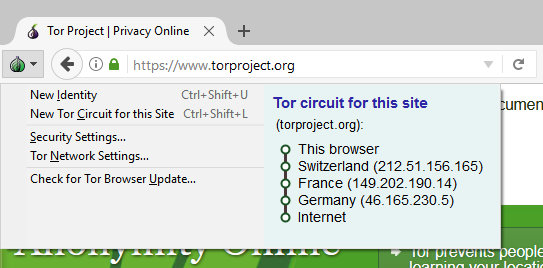
\includegraphics[width=\linewidth]{figures/tor-button-screenshot.jpg}
    \caption{A click on the onion icon reveals the Tor relays that constitute
    the circuit that was used to fetch the current page.}
    \label{fig:tor-button}
\end{figure}

Several of our participants enjoyed the visual feedback in Tor Browser (see
Figure~\ref{fig:tor-button}) that shows the circuit that is used for a given
site:

\begin{displayquote}
I love how I can monitor the network through this little kind of bar that
comes up.
\end{displayquote}

More generally, some participants wished it were easier to learn what is
happening behind the scenes:

\begin{displayquote}
{[It]} would be nice to have some kind of application, something on that browser,
that gives you an impression of\dots what the Tor Browser's actually doing.
\end{displayquote}

While the similarity of Tor
Browser's user interface to Firefox may be welcoming to newcomers, more
experienced users are struggling with the lack of feedback when sites don't
load:

\begin{displayquote}
\dots maybe some sort of graphical representation of is the circuit still
being built, or is the circuit built, and the site isn't responding at all to
the third relay?
\end{displayquote}

Crucially, some of our participants indicated that they originally started using
Tor Browser out of curiosity.  While these participants may appreciate more
visual feedback, other users who see Tor Browser as a mere tool to get the job
done may be overwhelmed by additional feedback.

\begin{displayquote}
In terms of the anonymity, you can't really tell\dots That's fairly opaque, so I
can't even tell how effective that's working, or whether it is\dots
\end{displayquote}

Several of our participants lamented the limited documentation.  Asked about the
difficulties of setting up an onion service, one participant responded:

\begin{displayquote}
Tor does a good job on their web site of telling you to modify your torrc file,
and then getting the onion set up.  But it's just very basic.  I have to go [to]
other people's blog post to find out.
\end{displayquote}

In addition to the lack of comprehensiveness of documentation, one participant
struggled with the lack of localization.  While Tor Browser's user interface is
available in Spanish, the documentation is not:

\begin{displayquote}
Think more [about] the Spanish community\dots because in my case I'm trying to
train people to use Tor but I work in the indigenous communities and there are
some things that [are] hard for me to explain in terms of how you use Tor\dots
\end{displayquote}

During our interviews we asked our participants to draw a sketch of how they
believe Tor and onion services work.  Everybody could draw a sketch of Tor but
some didn't draw onion services as they had no mental model for it.
Interestingly, all participants understood that Tor bounces network traffic
across several relays and that this is key to the anonymity Tor provides.  For
example, Figure~\ref{fig:tor-sketch} stems from a participant with no technical
background.  While the details are incorrect,\footnote{Tor circuits use the same
forward and backward path and default to three hops.} the sketch correctly
resembles that a Tor circuit contains several hops.

\begin{figure}[t]
    \centering
    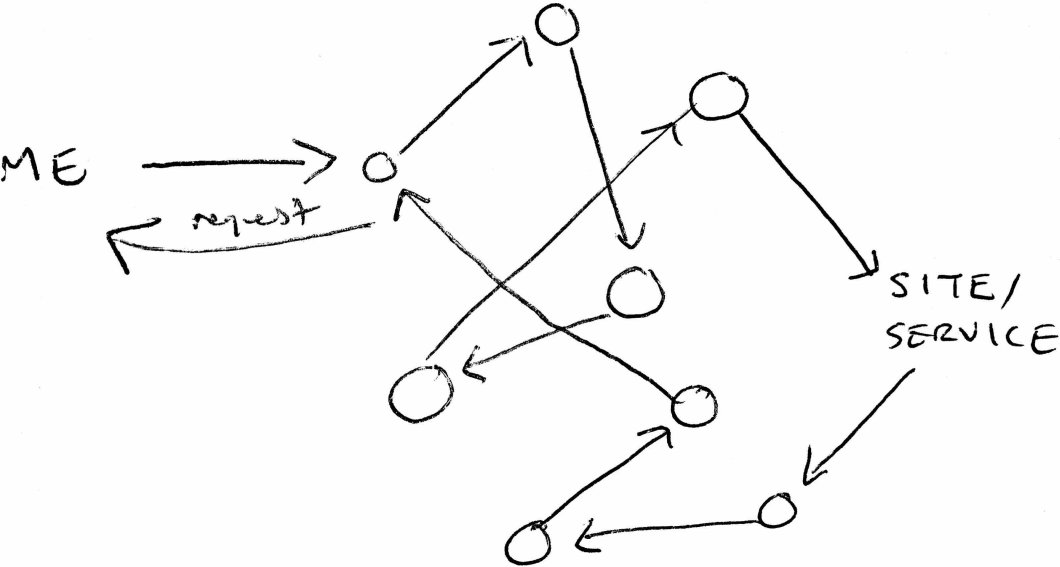
\includegraphics[width=0.8\linewidth]{figures/tor-sketch.jpg}
    \caption{A non-technical interview subject's sketch of how they believe Tor
    works.  The participant correctly understands the concept of bouncing
    network traffic over several hops.}
    \label{fig:tor-sketch}
\end{figure}

\begin{figure}[t]
    \centering
    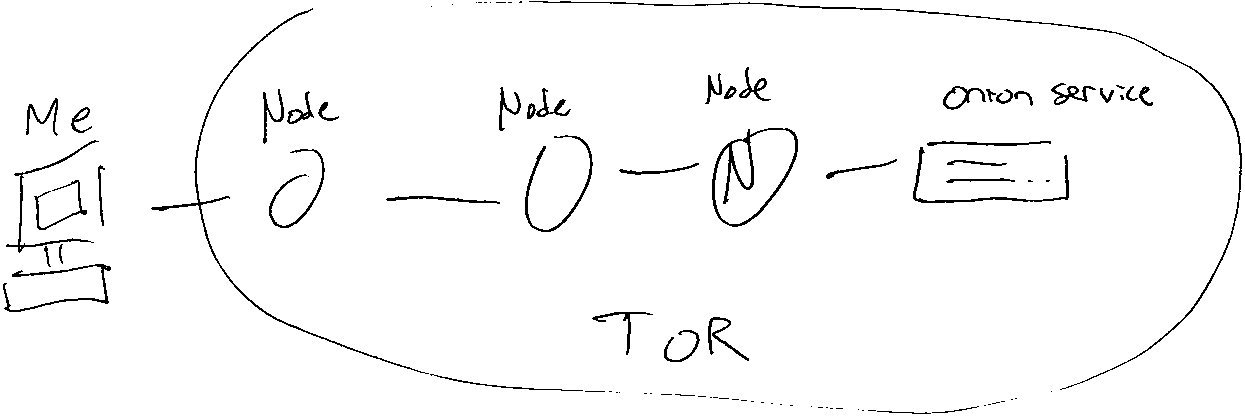
\includegraphics[width=0.8\linewidth]{figures/os-sketch.jpg}
    \caption{A non-technical interview subject's sketch of their mental model
    of an onion service.  Instead of a a web site, the final hop is another Tor
    hop.}
    \label{fig:os-sketch}
\end{figure}

\subsubsection{Misunderstandings}

Some statements of our participants suggested that they misunderstood aspects of
Tor.  A particularly common theme we encountered was the conflation of nuanced
aspects of anonymity.  Some of our participants did not distinguish between
anonymizing their identity and anonymizing the IP address.  There is still merit
in using Facebook's onion service.  While the company indeed learns who is
logging in, they will not learn their users' location and operating system, and
users get end-to-end security outside of the often brittle X.509 ecosystem as
well as self-authenticating names.  These concepts are difficult to convey to
users, however.  One participant voiced:

\begin{displayquote}
What's the point of going to Facebook using onion services when their business
model is still about collecting your data?
\end{displayquote}
Even technical users sometimes exhibit this ``all or nothing'' approach to
anonymity.

The domain format of onion services is a mystery to many users.  Some believe
that onion services are hidden \emph{because} their domains look random.
Therefore, they believe that vanity onion domains are ``less hidden'' because
part of their domain is not random.  Similarly, non-technical users have no
understanding of hash functions 

\subsubsection{Perception}

Public perception of The Tor Project and the work it does is heavily tied to
adoption.  Among our interview participants, The Tor Project enjoyed a lot
of trust:

\begin{displayquote}
Because, you guys\dots have the sort of\dots not a monopoly on trust, but you
have like a really great brand name when it comes to this stuff\dots
\end{displayquote}

Upon being told what an onion service is, one participant responded:

\begin{displayquote}
So it's like the Hidden Wiki and stuff like that, where you can buy drugs
and\dots or supposedly.
\end{displayquote}

Crime taking place over Tor and particularly on onion services was a common
theme.  Most of our participants feel safer when using Tor Browser instead of
another browser.  Some further distinguished between security and privacy, with
one respondent saying that ``\emph{Mozilla and Google do a lot for security but
    not for privacy}.''  Another participant 

\subsubsection{Disadvantages}

We were particularly interested in hearing what kind of issues Tor users face.
Perhaps the most common issue is (still) browsing speed:

\begin{displayquote}
The speed of it is problematic; sometimes I have a path that allows me to watch
streaming full HD YouTube videos, and the next time five minutes later I'm
barely getting kilobytes through.
\end{displayquote}

Occasionally, Tor's reputation precedes it and prepares users for what to
expect:

\begin{displayquote}
I didn't think it was as slow as people say it was. People said it would be much
slower experience but\ldots a little bit slower, but it didn't matter for the
things that I was doing.
\end{displayquote}

In addition to the perceived slowness, several participants lamented the
old-fashioned user interface.  Tor Browser's looks were described as
``\dots\emph{it felt like it was about five years outdated},'' ``\dots\emph{it
looked like I was in 1982},'' and ``\emph{I think the colors look a bit old
fashioned and in the former Soviet Union}\dots''

Many of our participants expressed concern that their use of Tor makes them
``stick out'' or paints a target on their backs.  Asked about the disadvantages
of using Tor, one participant responded:

\begin{displayquote}
The fact that you're using Tor.  So I think that alone to [an]\dots experienced
observer might be cause in some countries to ring your doorbell and ask what
you're up to.
\end{displayquote}

Another participant expressed this concern for other privacy tools as well:

\begin{displayquote}
When you have it on your laptop, for some authorities, that is a reason to think
of you as somebody who's deserving of suspicion.  Same thing when you have
Signal, or when you use PGP, just by having [these] that means that they
sometimes are inclined to think that, ``Oh you must have something to hide
because you've used these kind of technologies.''
\end{displayquote}

Interestingly, one participant expressed that the antiquated user interface
evoked trust:

\begin{displayquote}
At the same time I thought I think that it gave them a certain amount of
credibility, like they weren't building this for the looks, but they were
building it for functionality, so what it did.  At the same time, as I thought
it was outdated in terms of how it looked, I also thought it was sort of genuine
in a way.
\end{displayquote}

In 2016, Khattak \ea documented how Tor users are often treated differently than
non-Tor users~\cite{Khattak2016a}.  One participant mentioned:

\begin{displayquote}
It is still sometimes challenging using some everyday services, because of
CAPTCHAs and those things, but I also understand that's not so much to do with
Tor, but to do with the creators of those web sites.
\end{displayquote}

\subsubsection{Advantages}

\begin{displayquote}
I feel like I'm more in control of my internet experience that way, I'm not sort
of like a will-less victim of what other people want to do with me, so I feel
I'm more empowered and have more agency when I use the Tor Browser.
\end{displayquote}
